\documentclass{article}
%==============================================================================%
%	                          Packages                                     %
%==============================================================================%
% Packages
\usepackage[utf8]{inputenc}
\usepackage{graphicx}
\usepackage{amsmath}
\usepackage{amssymb}
\usepackage{braket}
\usepackage[margin=0.7in]{geometry}
\usepackage[version=4]{mhchem}
\usepackage{url}
\usepackage{float}
%==============================================================================%
%                           User-Defined Commands                              %
%==============================================================================%
% User-Defined Commands
\newcommand{\be}{\begin{equation}}
\newcommand{\ee}{\end{equation}}
\newcommand{\benum}{\begin{enumerate}}
\newcommand{\eenum}{\end{enumerate}}
\newcommand{\pd}{\partial}
\newcommand{\dg}{\dagger}
%==============================================================================%
%                             Title Information                                %
%==============================================================================%
\title{Chem237: Lecture 6}
\date{4/12/18}
\author{Shane Flynn}
%==============================================================================%
%==============================================================================%
\begin{document}
\maketitle
\section*{Extreme Integration}
Start with Taylor Series.

If f(z) is regular in D, than all derivitives exist, therfore we can expand f(z) in a taylor series about some point z$_0$. 
\be
\begin{split}
    a &= f(z_0)\\
    a_n &= \frac{1}{n!} f^n(z_0)
\end{split}
\ee

The question is if the series converges?
If z$_0$ is in the center of a disk iwth radius r, such that r is equal to the distance between z$_0$ and teh closest singularity. 

\begin{figure}[H]
  \centering
    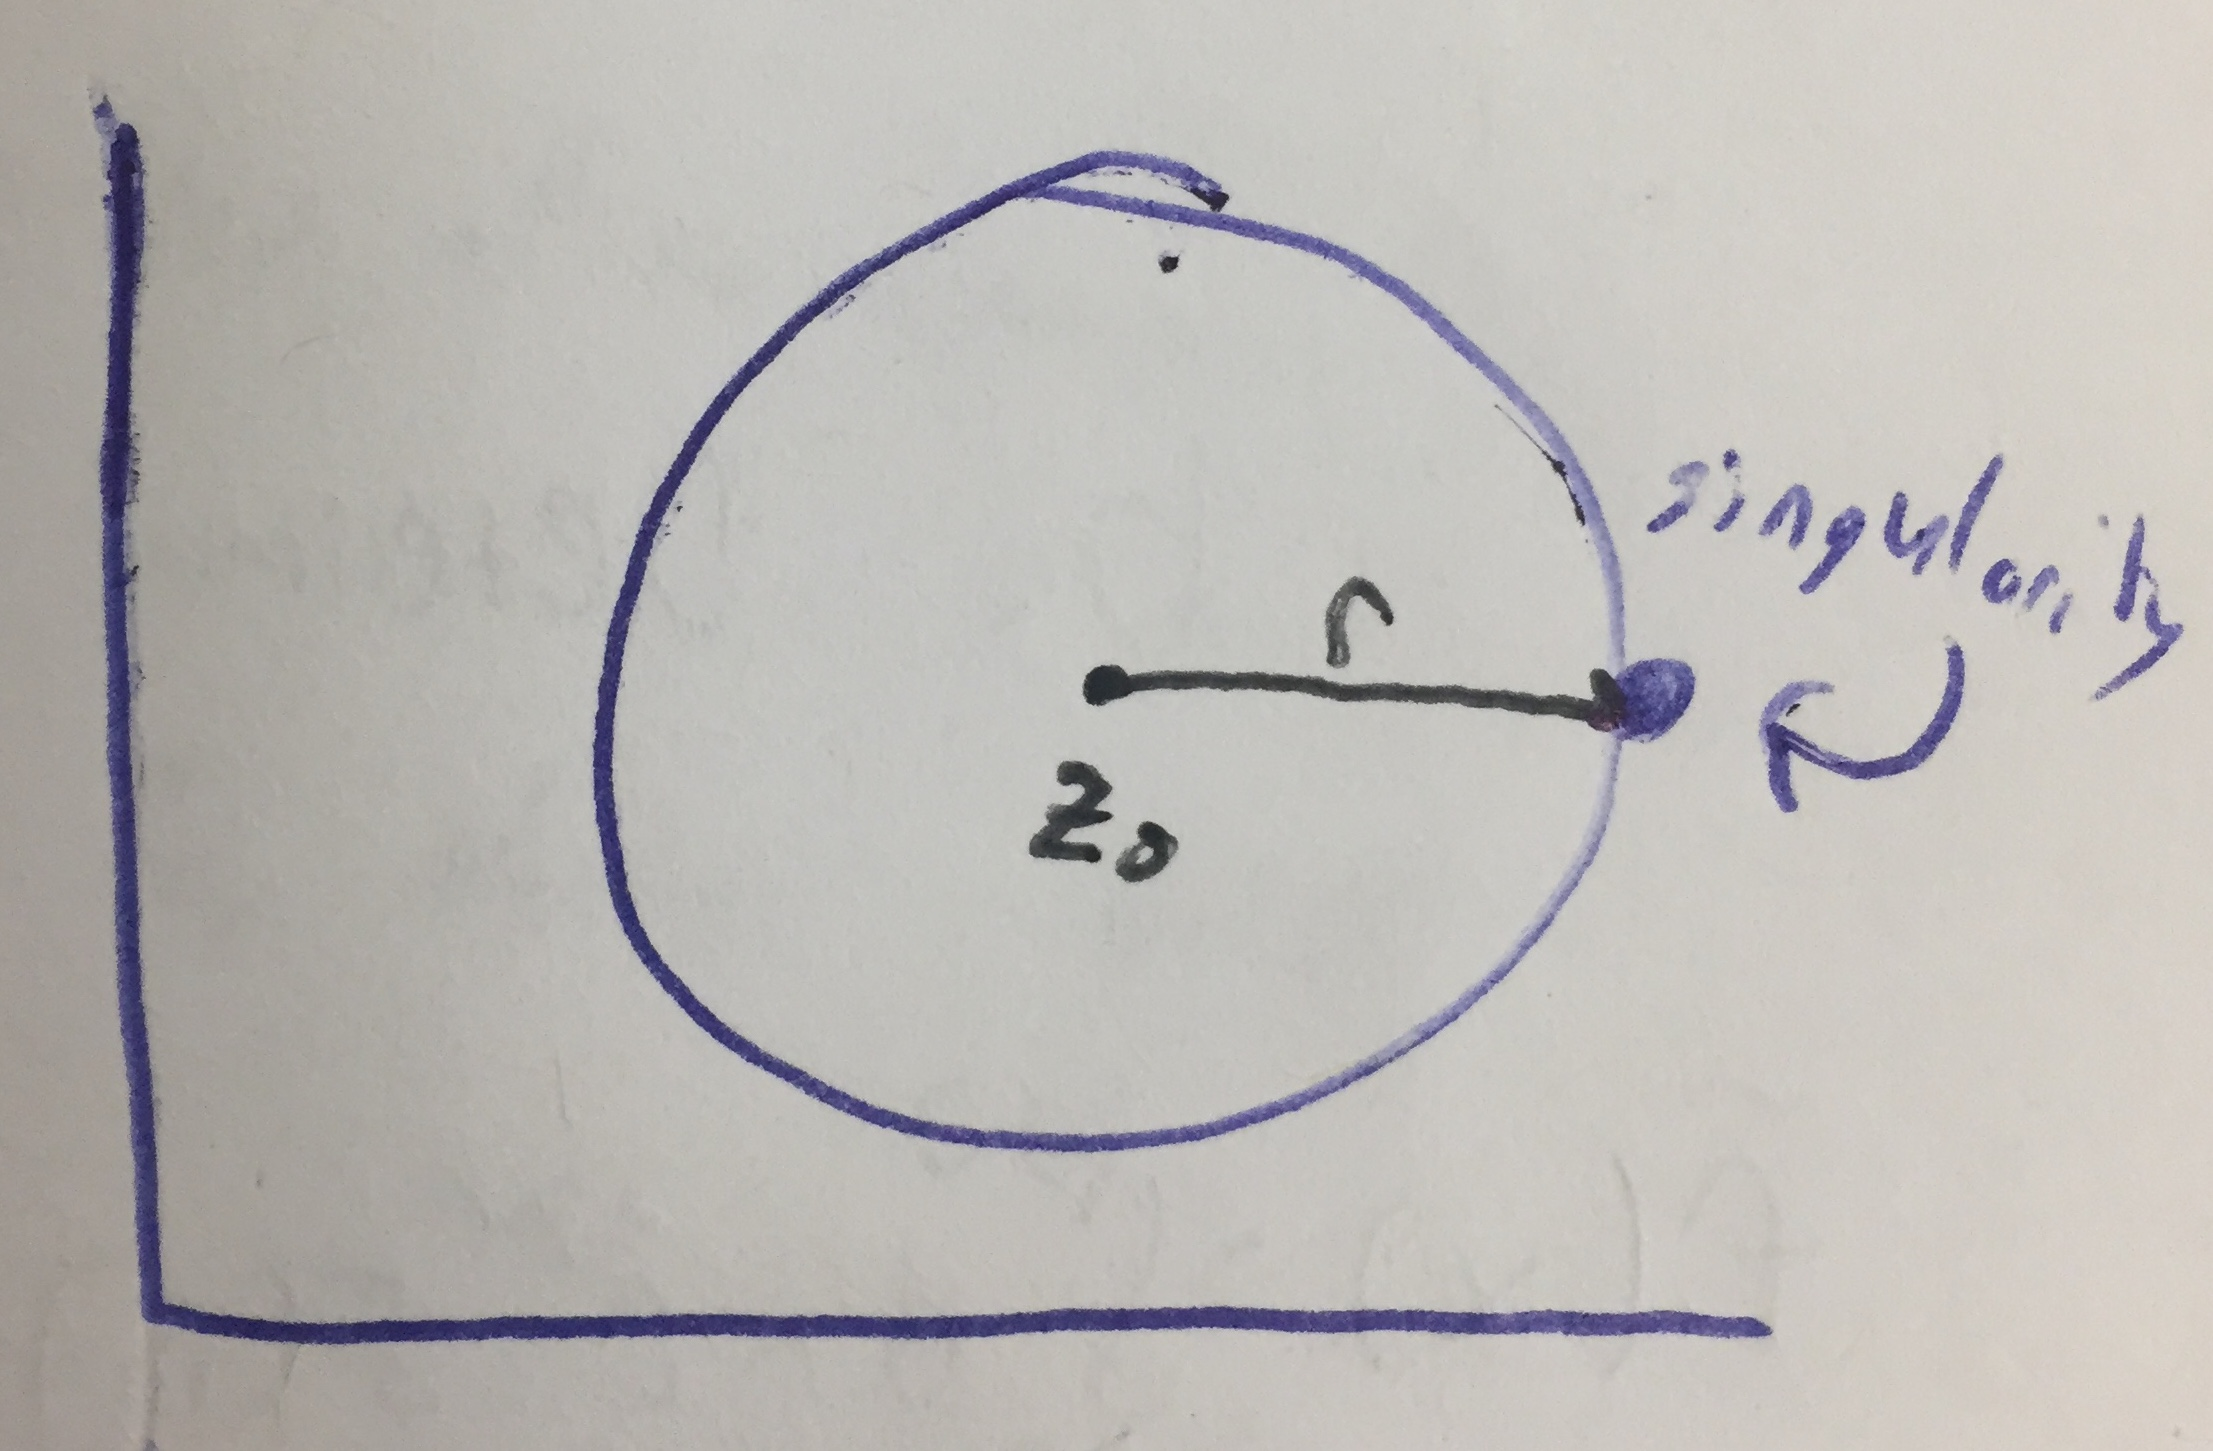
\includegraphics[scale=0.2]{Figures/converge.png}
    \caption{Make a caption. Radius of Convergence defined by r. R is length to closest singulaiity.}
\end{figure}

As an example consider 
\be
f(z) = \frac{1}{z}
\ee
The function exists everywhere, except for the singulairty at z=0. 
To evaluate we can expand the funciton
\be
\frac{1}{z} = \frac{1}{1-\left(\frac{z_0-z}{z_0}\right)^n}
\ee
We can now use a geometrix series
The Taylor series is
\be
\frac{1}{z_0} \sum_{n=0}^\infty \left(\frac{z_0-z}{z_o}\right)^n
\ee
To convege then 
\be
\frac{z-z_0}{z_0}< 1
\ee
We know z-z$_0 < z_0$. 

\subsection*{Laurent Series}
Expand the series about point z$_0$
\be
\begin{split}
    f(z) &= \sum_{n=-\infty}^\infty a_n (z-z_0)^n\\
    a_n &= \frac{1}{2\pi i} \oint_\gamma dz \frac{f(z)}{(z-z_0)^{n+1}}
\end{split}
\ee
Where teh second line comes from cauchy. 

As an example we can again use f(z) = $\frac{1}{z}$ whih is naturally the form for a laurentz series.
\be
\frac{1}{z} =\frac{a_1}{z-0}
\ee
Where we define a$_1$ = 1 and z$_0$ = 0

The contour would need to go around z$_0$, but we may not need to include z$_0$ in our domain (i.e. we can make the contour as small as we want around z$_0$ infinately small about the point. 
\begin{figure}[H]
  \centering
    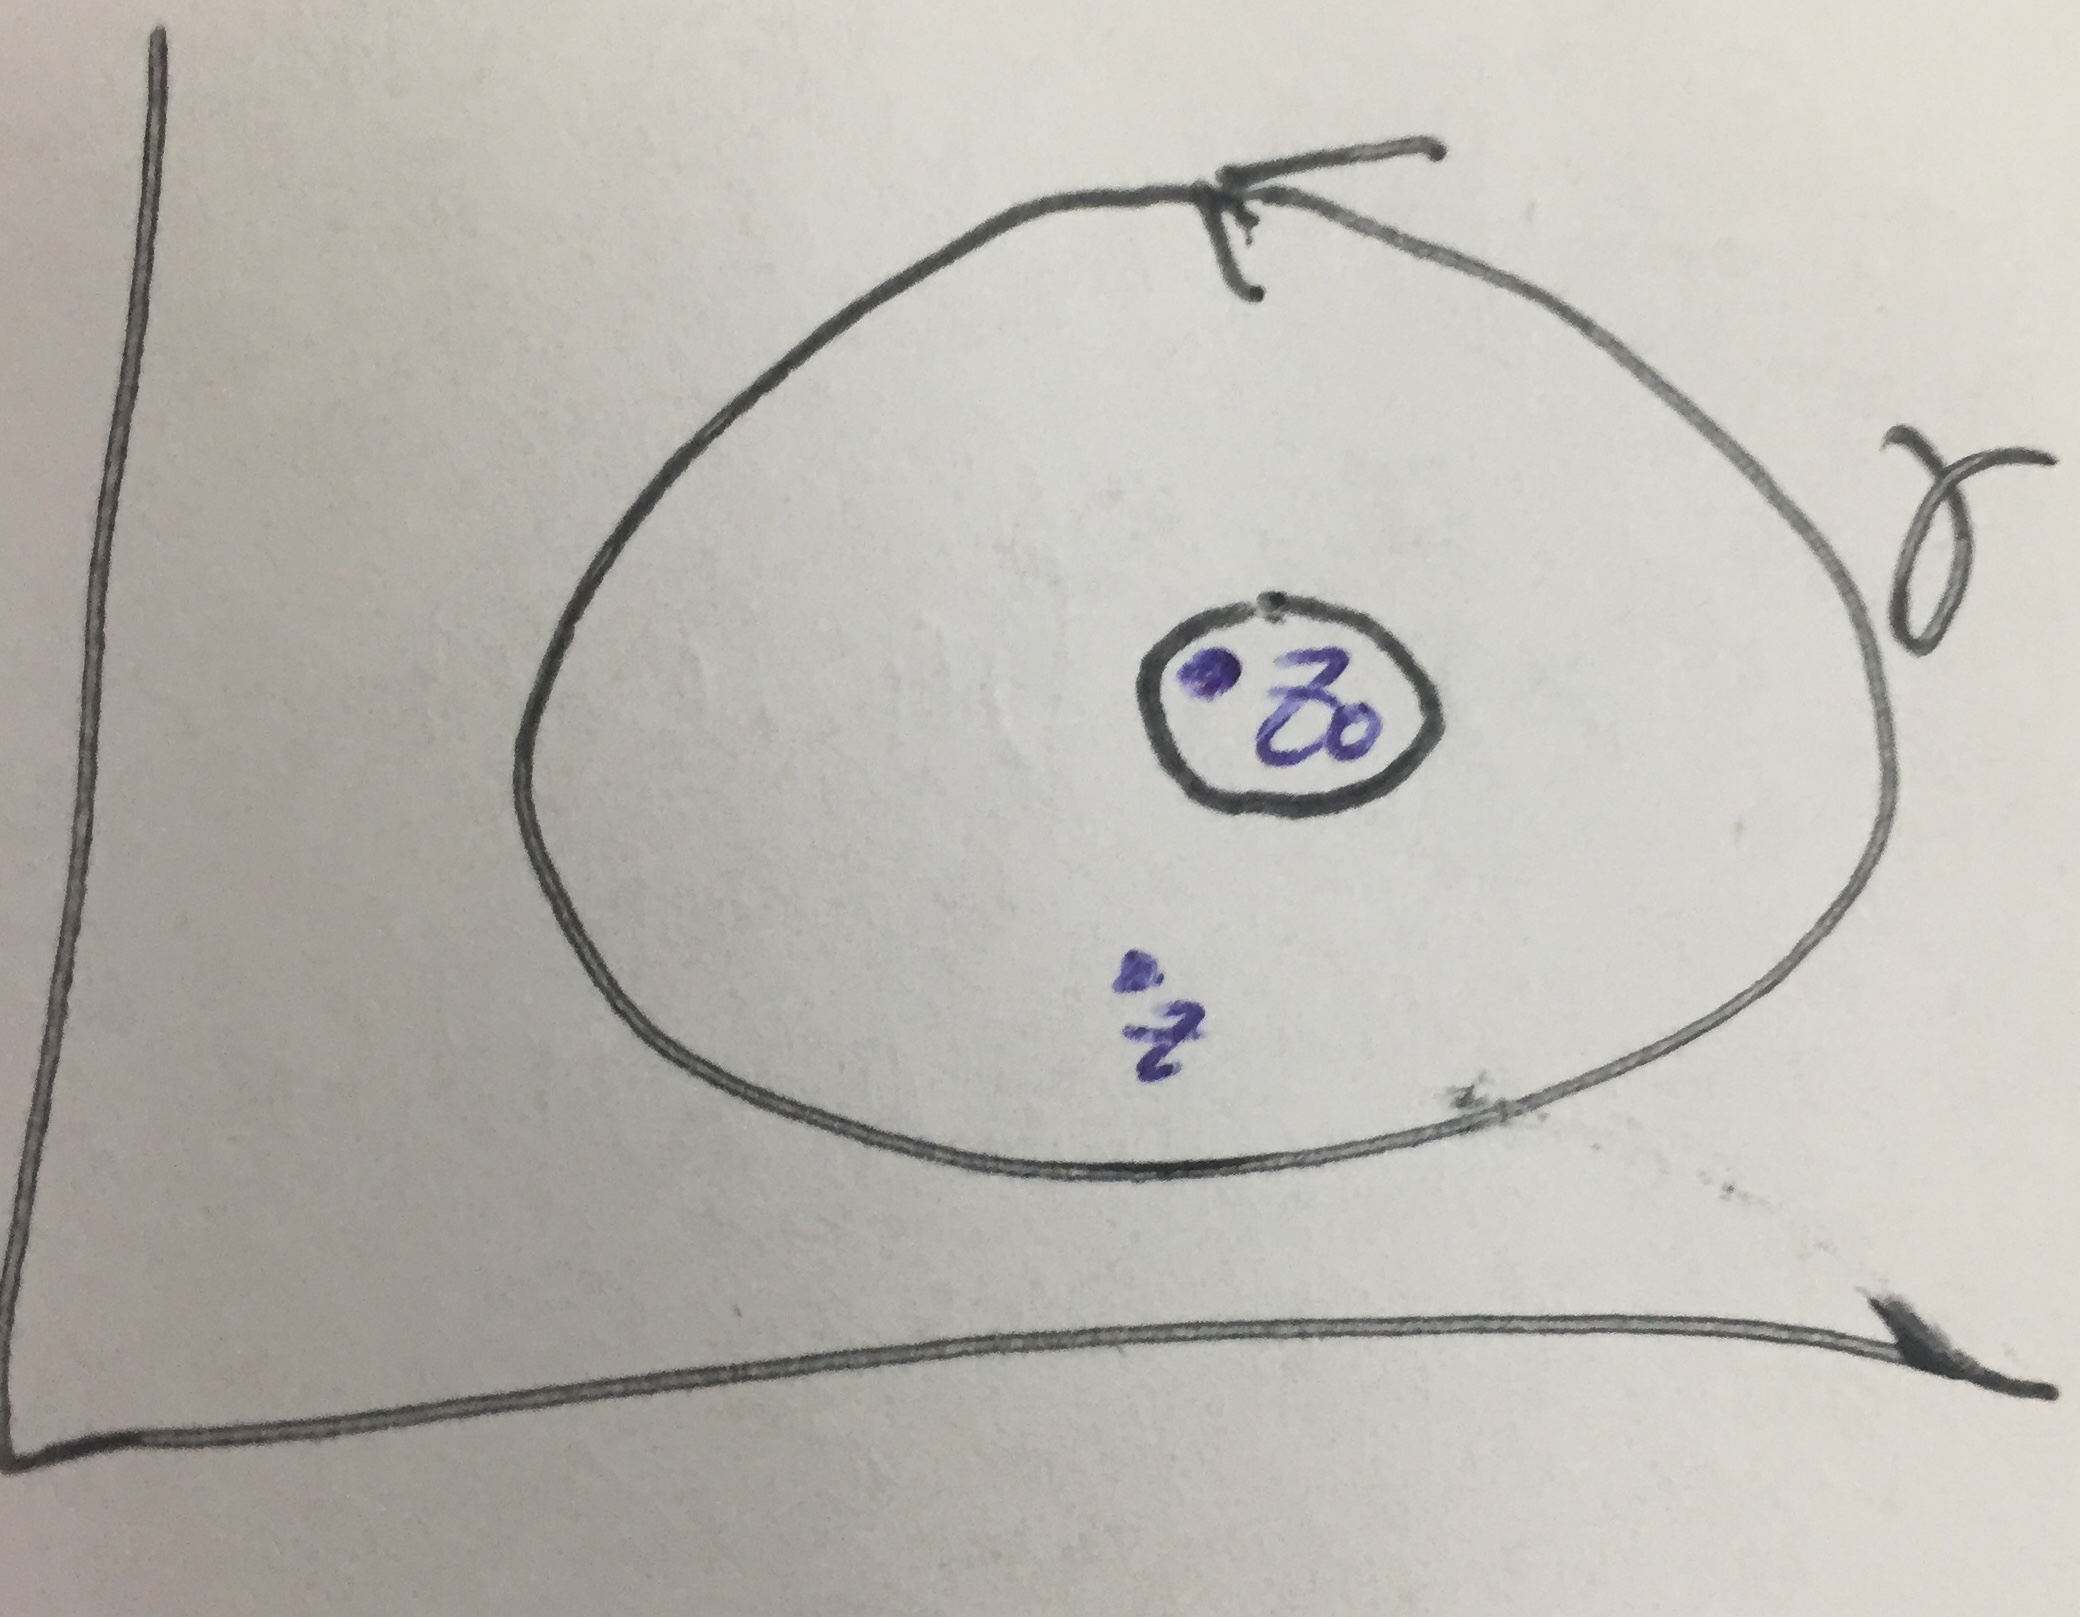
\includegraphics[scale=0.2]{Figures/laurent.png}
    \caption{Make a caption. Radius of Convergence defined by r. R is length to closest singulaiity.}
\end{figure}

We can now represent f(z) at any point z because the function is regular the integral is not a function of path. 

\subsection*{Pole}
z$_0$ is a simple pole of order M if a$_m \neq 0$, but for any m'$>$m a$_{m'}$=0.

If m is infinite, than z$_0$ is known as a essential singularity at this point. 

There are other types of singularities, ofr example  abranching point occurs for f(z) = $\sqrt{z}$. 
In polar coordinates we could write z = Re$^{i\theta}$. 
\be
    f(z) = \sqrt{z} = \sqrt{R}e^{i\theta}
    \ee
We can choose a new contour
\begin{figure}[H]
  \centering
    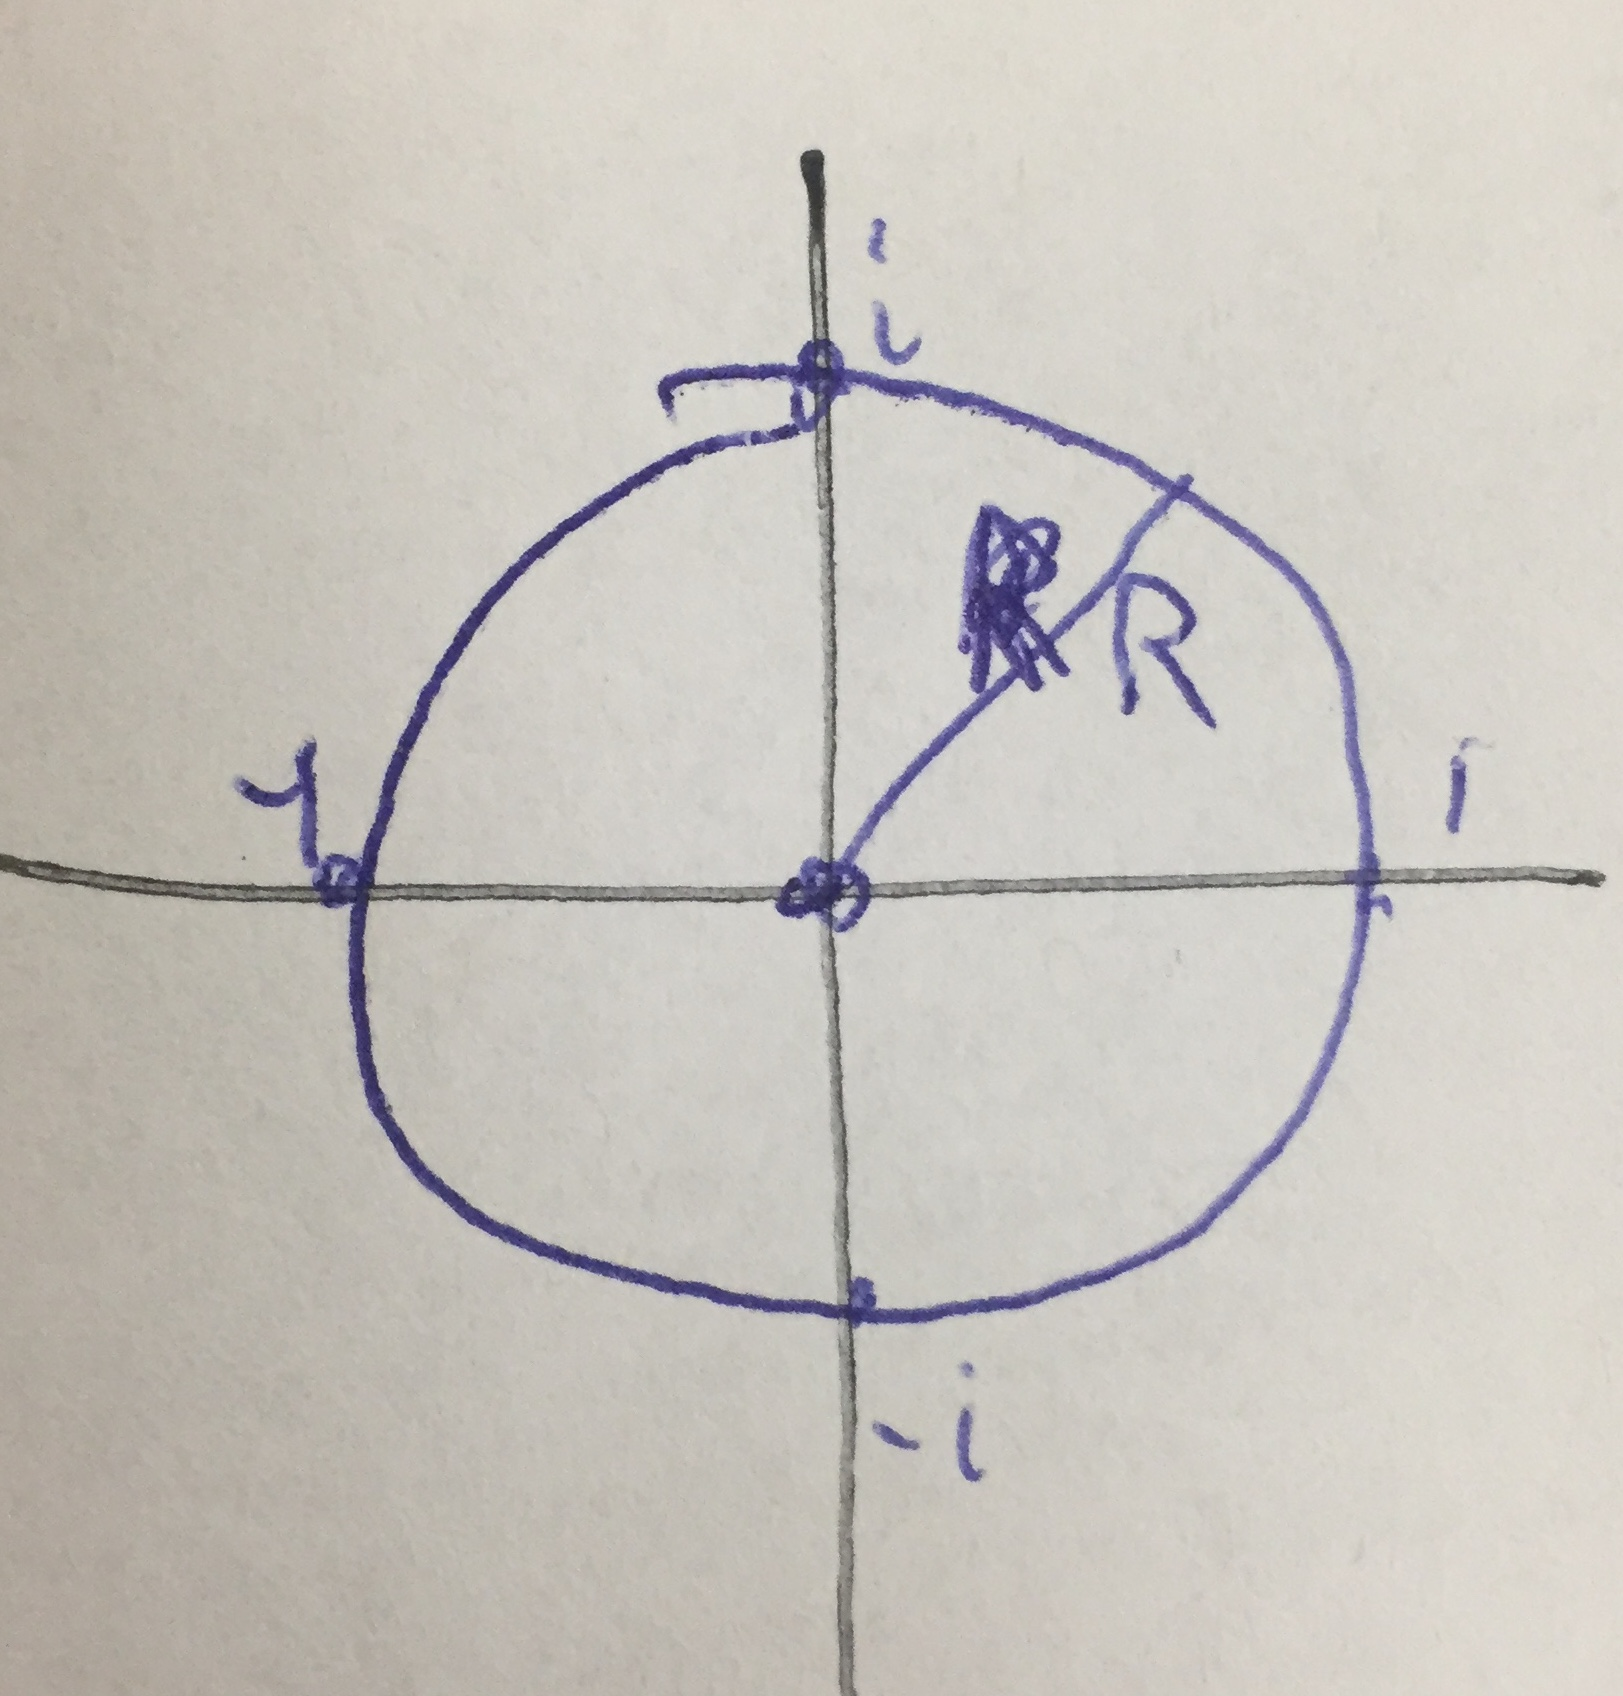
\includegraphics[scale=0.2]{Figures/circle.png}
    \caption{Make a caption. Radius of Convergence defined by r. R is length to closest singulaiity.}
\end{figure}
\be
\begin{split}
    f(1) &= e^{i\theta/2} = 1\\
    f(i) &= e^{i\pi/4} = 1\\
    f(-1) &= e^{i\pi/2} = 1\\
    f(1) &= e^{i2\pi/2} = -1\\
\end{split}
\ee
The function continuously changes about the branching point, start at 1, end at -1, the function therefore cannot be continuous. 
If you go around another time, you will get a value of 1, and so on.
This means $\sqrt{z}$ is a double-value function.


We can consider instead $\ln(z)$, and again let z=$Re^{i\theta}$, recall n=$\pm$ (1,2,3,..). 
\be
\begin{split}
    f(z) &= \ln(z) = \ln(Re^{i\theta}) = \ln(Re^{i\theta+2\pi ni}) = \ln(R) + \ln(e^{i\theta + 2\pi in})\\
    &= \ln(R) + 2\pi ni + i\theta
\end{split} 
\ee
Therefore ln is an infinite valued function (because n runs from 0 to infinity), we collect a phase each iteration
\be
\begin{split}
    \ln(1) &= 0\\
    \ln(2) &= 2\pi i\\
\end{split}
\ee

Another tyoe of singularity is an esseintail singularity, consider a Taylor expansion.
\be
f(z) = e^{1/z} =n\sum_{n=0}^\infty \frac{1}{n!}\frac{1}{z^n}
\ee
All the a$_n$ terms are $\frac{1}{n!}$ so they all exist, z=0 is an essential singularty. 

\section*{The Residue Theorem}
\be
\oint dz \quad f(z) = 2\pi i\sum_i \text{res}
\ee

Consider some function f(z) in a domain D, with isolated residues z$_1$, z$_2$, ...

\begin{figure}[H]
  \centering
    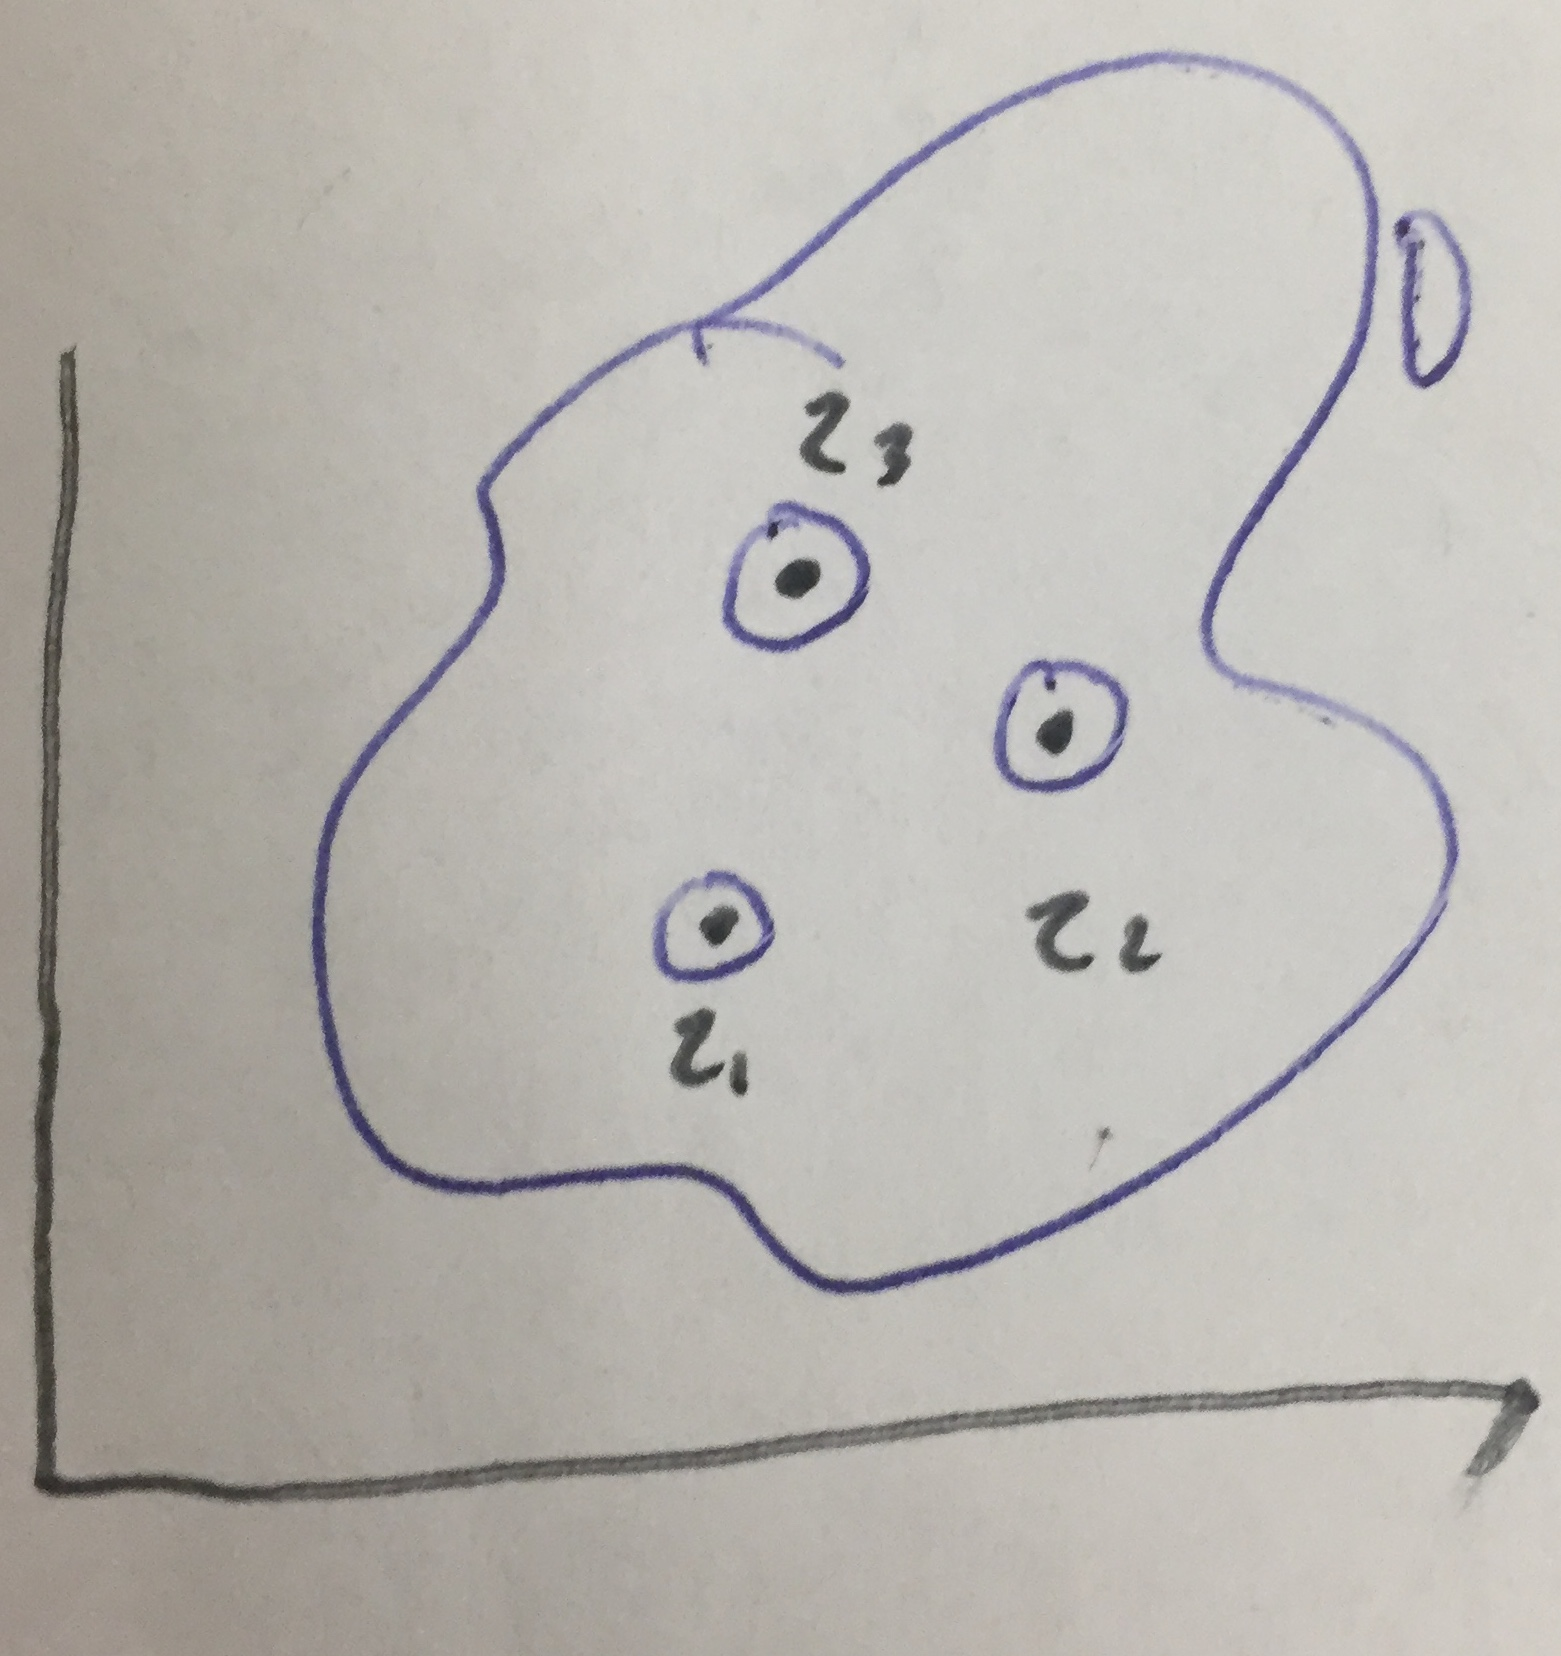
\includegraphics[scale=0.2]{Figures/res.png}
    \caption{Make a caption.isolated singularities} 
\end{figure}

If you define a contour over a set of isolated isngularities (poles) than the value of the integral is simply the values associated with the singularities through the residue theorem. 

\be
\text{residue} = \lim_{z \rightarrow z_0}{(z-z_0)} = a_1(z_0) \Rightarrow \lim_{z \rightarrow z_0}{f(z)} \frac{a_1}{(z-z_0} \Rightarrow a_1(z_0) = \text{residue}
\ee

So you need to cmpute a limit for each singularity to get the residue, and compute the integral through all of the residues. 

\subsection*{Isolated Singularities}
There own tyoe of singularity (finite power), these methods do not work forbranching points and esenitial  singularities, keep that in mind. 

As an example consider
\be
f(z) = \frac{e^z}{z^5} \Rightarrow \oint dz \quad \frac{e^z}{z^5}
\ee

We can expand e$^z$ using a Taylor series
\be
\oint dz \quad \frac{e^z}{z^5} = \oint dz \quad \frac{1}{z^5} \left(1+z+\frac{z^2}{2!} + \cdots\right) = \oint dz \quad 
\ee
We could then try to compute this integral using a laurentz series (he did not actually do this example may want ot remove
\be
\oint dz \quad \left(\frac{1}{z^5} + \frac{1}{z^4} + \frac{1}{2!z^3} + \frac{1}{4!z} + \frac{1}{5!} + \frac{z}{6!} + \cdots \right)
\ee

This is some extreme integration according to Vlad, but we can actually solve the problem a bit easier.
The Laurent series is unique, and it turns out only the $\frac{1}{4!z}$ term actually contributes, all other terms go to 0.
Therefore we do not actually need a Laurentz series, we can just use the Residue Theorem. 

Consider instead
\be
\begin{split}
    \oint_\mathbb{C} & dz \quad \frac{1}{z^n} \\
    z = Re^{i\theta}, \quad & \quad dz = iRe^{i\theta}d\theta \\
    \oint_\mathbb{C} & d\theta \quad ie^{i(1-n)\theta} \\
    &= \begin{cases}
   2\pi i, & \text{if $n=1$}\\
    0, & \text{otherwise}.
  \end{cases}
\end{split}
\ee
So we see that our extreme integration terms evaluate to z if n$\neq$1, so we only need to compute a single term. 
\be
\oint dz \quad \frac{e^z}{z^5} = 2\pi i a_1(z=0)
\ee
We don't need to solve the integral, we just need to compute the residue and evaluate at that point, no need for our laurent series at all. 

\subsection*{Integrals}
The class of integrals that can be evaluated through the residue theorem is very broad, with both defininte and indefinite integrals included.

Consider the following integral
\be
\int_0^\infty dx \quad \frac{\cos(x)}{1+x^2}
\ee
It is usually convenient to replace trig functions with their expotential representation, cos(x) = Re$\left[e^{iz}\right]$, we can re-write the above integral as
\be
Re\int_0^\infty dz \quad \frac{e^{iz}}{1+z^2}
\ee
This expression contains isolated singularities at $\pm$i, these are simple poles (absolute singularities). 
We can draw our contour over one of these poles as

\begin{figure}[H]
  \centering
    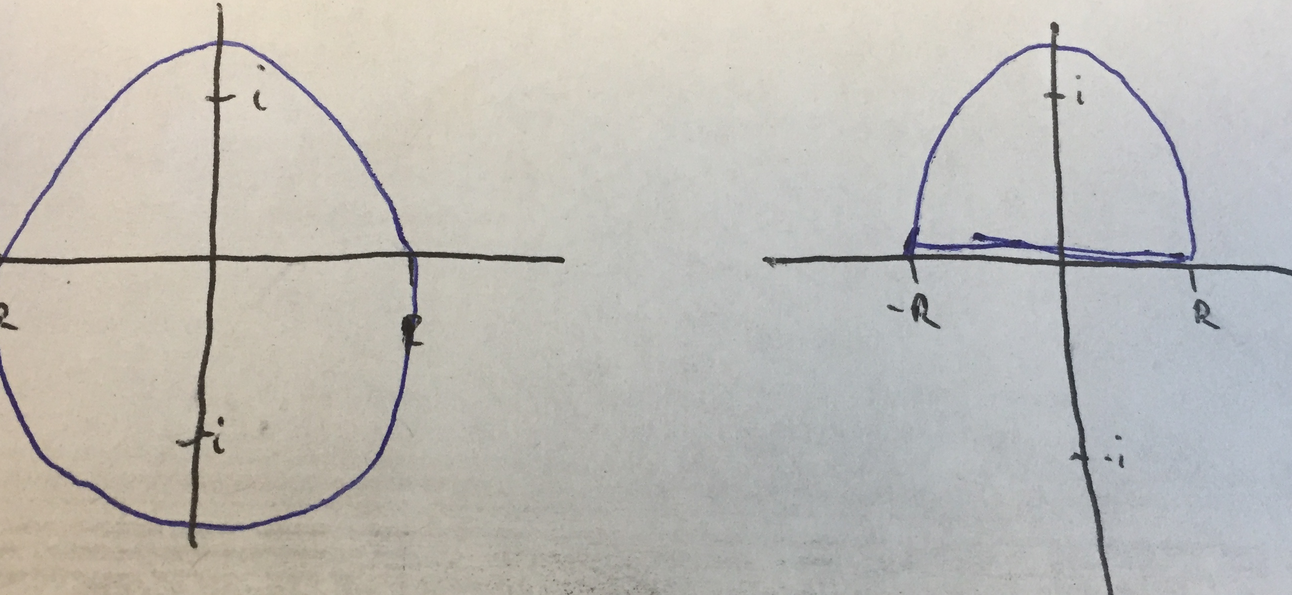
\includegraphics[scale=0.2]{Figures/example.png}
    \caption{Make a caption.Two poles at $\pm$i, both contours are valid, but the right 1 is easier to evaluate, only need to compute 1 residue. WE NEED TO LABEL PATHS  AROUND THE CONTOUR!!!!!}
\end{figure}

Ths integral can be computed using the residue theorem.
Using the figure on the right our original integral is a summation of two terms, the curve in teh complex plane and the line across the real axis (which is our line integral of interest). 
It will be more convenient to change the bounds of our original integral as we will see, using the fact that this integral is for an even function we cna write
\be
\int_0^\infty dx \quad \frac{\cos(x)}{1+x^2} = \frac{1}{2} \int_{-\infty}^\infty dx \quad \frac{\cos(x)}{1+x^2}
\ee
To comput our residue at i comsinder
\be
\begin{split}
    \text{res}(z=i) &=  \lim_{z \rightarrow i}{\frac{e^{iz}}{1+z^2}(z-i)}\\
    &=  \lim_{z \rightarrow i}{\frac{e^{iz}}{(z-i)(z+i)}(z-i)}\\
    \text{res}(z=i) &= \frac{e^{-1}}{2i}
\end{split}
\ee
Using our residue we can not comput eour integral of interest (cosine is the real part of the expotential representation). 
\be
Re\left[\int_0^\infty dz \quad \frac{e^{iz}}{1+z^2}\right] = 2\pi i \text{Res}(z=i) = \frac{\pi}{e}
\ee

From our diagram we are computing an integral over our closed contour.
Pathway I is the real integral of interest we are asked about in the question, and we used the residue theorem to compute the integral over the entire contour.
This means that path II must evaluate to zero for our contour integral to be equal to the original question we awere asked.
So we need to evaluate integral II explicitly, it is a semi-circle so we can naturally switch coordinates.
\be
\begin{split}
    II &= \int_{-R}^R dz \quad \frac{e^{iz}}{1+z^2}\\
    z = Re^{i\theta}, \quad dz = & Rie^{i\theta}d\theta, \quad iz = iz + i^2y = ix-y\\
    &= \int_0^\pi d\theta \quad Rie^{ix-y} \frac{e^{i\theta}}{i1+R^2e^{2i\theta}}\\
    &= \lim_{R \rightarrow \infty}{\left[\int_0^\pi d\theta \quad Rie^{ix-y} \frac{e^{i\theta}}{i1+R^2e^{2i\theta}}\right]} = 0
\end{split}
\ee
Where the limit is much easier to evaluate at the limit to infinity, becuae this term goes to 0, the vlaue of the residue theorem is exactly equal to the interal over the real line (the original question we were asked). 
%%%%%%%%%%%%%%%%%%%%%%%%%%%%%%%%%%%%%%%%%%%%%%%%%%%%%%%%%%%%%%%%%%%%%%%%%%%%%%%%%%%%%%%%%%%%%%%%%%%%%%%%%%%%%%%%%%%%%%%%%%%%%
% IF I FELT MOTIVATED I SHOULD SHOW YOU GET THE SAME ANSWER WITH CONTOUR OVER BOTH POLES
%%%%%%%%%%%%%%%%%%%%%%%%%%%%%%%%%%%%%%%%%%%%%%%%%%%%%%%%%%%%%%%%%%%%%%%%%%%%%%%%%%%%%%%%%%%%%%%%%%%%%%%%%%%%%%%%%%%%%%%%%%%%%

\subsubsection*{Another Example}
%%%%%%%%%%%%%%%%%%%%%%%%%%%%%%%%%%%%%%%%%%%%%%%%%%%%%%%%%%%%%%%%%%%%%%%%%%%%%%%%%%%%%%%%%%%%%%%%%%%%%%%%%%%%%%%%%%%%%%%%%%%%%
%%%%%%%%%%%%%%%%%%%%%%%%%%%%%%%%%%%%%%%%%%%%%%%%%%%%%%%%%%%%%%%%%%%%%%%%%%%%%%%%%%%%%%%%%%%%%%%%%%%%%%%%%%%%%%%%%%%%%%%%%%%%%
%%%%%%%%%%%%%%%%%%%%%%%%%%%%%%%%%%%%%%%%%%%%%%%%%%%%%%%%%%%%%%%%%%%%%%%%%%%%%%%%%%%%%%%%%%%%%%%%%%%%%%%%%%%%%%%%%%%%%%%%%%%%%
% Shwo out all work for this problem 
Consider the following integral (Assume a is positive). 
\be
\int_{-\infty}^\infty dx \quad \frac{x\cos(ax)}{1+x^2}
\ee

Again we start by drawing a contour, this problem is similar to the last, the residues occur at plus or minus i so we can use the same semi-circle contour as above.
\be
\begin{split}
    \int_{-\infty}^\infty dx \quad \frac{x\cos(ax)}{1+x^2} &= I + II\\
    \int_{-\infty}^\infty dx \quad \frac{x\cos(ax)}{1+x^2} &=  Re\left[\lim_{R \rightarrow \infty}{\left(\oint dz \quad \frac{ze^{iaz}}{1+z^2}\right)} \right]+ Re\left[\oint d\theta \quad \frac{R^2ie^{aix-ay}e^{2i\theta}}{1+R^2e^{zi\theta}} \right]
\end{split}
\ee
If you check (wolfram) the limit for the final integral does go to 0, so we can solve this problem using the residue theorm just like in the previous example. 

Using the residue theorem we can com pute our remaining integral
\be
\text{res}(i) = \frac{ie^{iai}}{1+i^2}(1-i) = \frac{e^{-a}i}{1+i} \rightarrow -2\pi \frac{e^a}{1+i}
\ee
% Need to fully do out this problem and show how to solve better^^^^^^^^^^^^^^^^^^^^^^^^^^^^^^^^^^^^^^^^^^^^^^^^^^^^^^^^^
%%%%%%%%%%%%%%%%%%%%%%%%%%%%%%%%%%%%%%%%%%%%%%%%%%%%%%%%%%%%%%%%%%%%%%%%%%%%%%%%%%%%%%%%%%%%%%%%%%%%%%%%%%%%%%%%%%%%%%%%%%%%%
%%%%%%%%%%%%%%%%%%%%%%%%%%%%%%%%%%%%%%%%%%%%%%%%%%%%%%%%%%%%%%%%%%%%%%%%%%%%%%%%%%%%%%%%%%%%%%%%%%%%%%%%%%%%%%%%%%%%%%%%%%%%%
%%%%%%%%%%%%%%%%%%%%%%%%%%%%%%%%%%%%%%%%%%%%%%%%%%%%%%%%%%%%%%%%%%%%%%%%%%%%%%%%%%%%%%%%%%%%%%%%%%%%%%%%%%%%%%%%%%%%%%%%%%%%%






\end{document}
